\newprob{lqone}{
    小新(以箭號AB 表示)站在垂直平面鏡(MN)前 2 m 的位置。已知他高160 cm,眼睛(E) 離地面 150 cm。\\Sam (arrow AB) of height 160 cm is standing 2 m in front of a vertical plane mirror (MN). His eyes (E) are 150 cm above the ground.\bigskip
    {\par\centering
        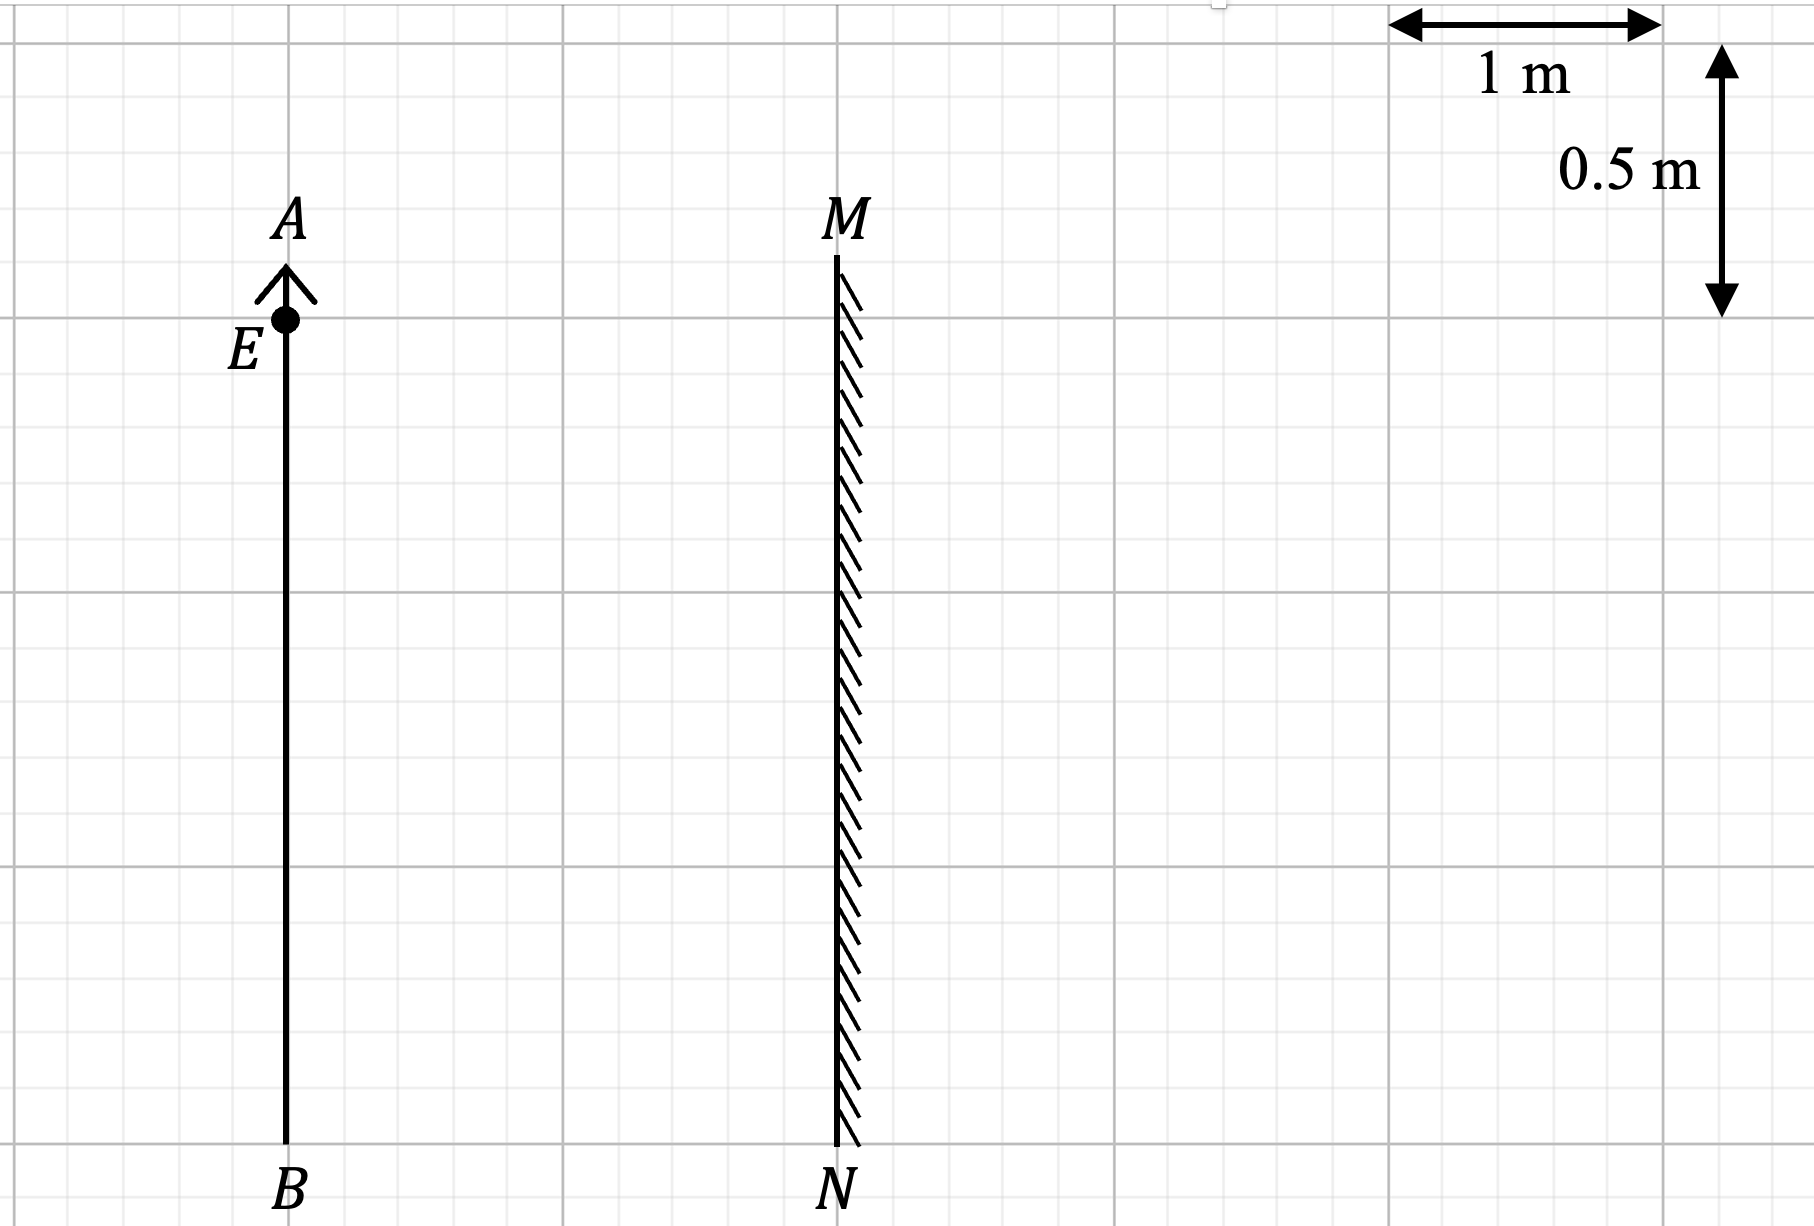
\includegraphics[width=0.75\linewidth]{dq9812us.png}\par}
    \bigskip
    \begin{parts}
        \part \begin{subparts}
            \subpart 試在方格紙上繪畫光線圖,以表示小新 如何在鏡中看見自己的全身像。\\Draw, on the graph paper, a ray diagram to show how Sam sees his whole body in the mirror. \par\zh{2}
            \subpart 由此或以其他方法,求鏡子足以讓小新 看見自己的全身像最小長度。 \\Hence, or otherwise, find the min. length of the mirror such that Sam can see his whole body. \par\zh{1}
            \dlines{1}
            \subpart 若小新向鏡子走近數步,(ii)的答案會 有何變化? \\How would the answer in (ii) change if Sam moves a few steps towards the mirror? \zh{1}
            \dlines{1}
        \end{subparts}

        \clearpage
        \part 小新的攣生兄弟小銘起初站在小新旁邊。現在小銘向走向小新正前方 0.5 m 處。\\Mike, who is an identical twin of Sam, was standing besides Sam, now is 0.5 m right in front of Sam.
        \begin{subparts}
            \subpart 小銘若要看見小新的全身像,鏡子的最 小長度是多少? \\What is the min. length of the mirror for Mike to see the whole body of Sam?\zh{2}
            \dlines{1}
            \subpart 小銘認為若他後退數步,(i)的答案會變 小。你同意嗎?試扼要解釋。 \\Mike thinks that the answer in (i) would be smaller if he moves a few steps backwards. Do you agree? Explain briefly.\zh{2}
            \dlines{1}
        \end{subparts}
    \end{parts}

}
{
    {\par\centering
            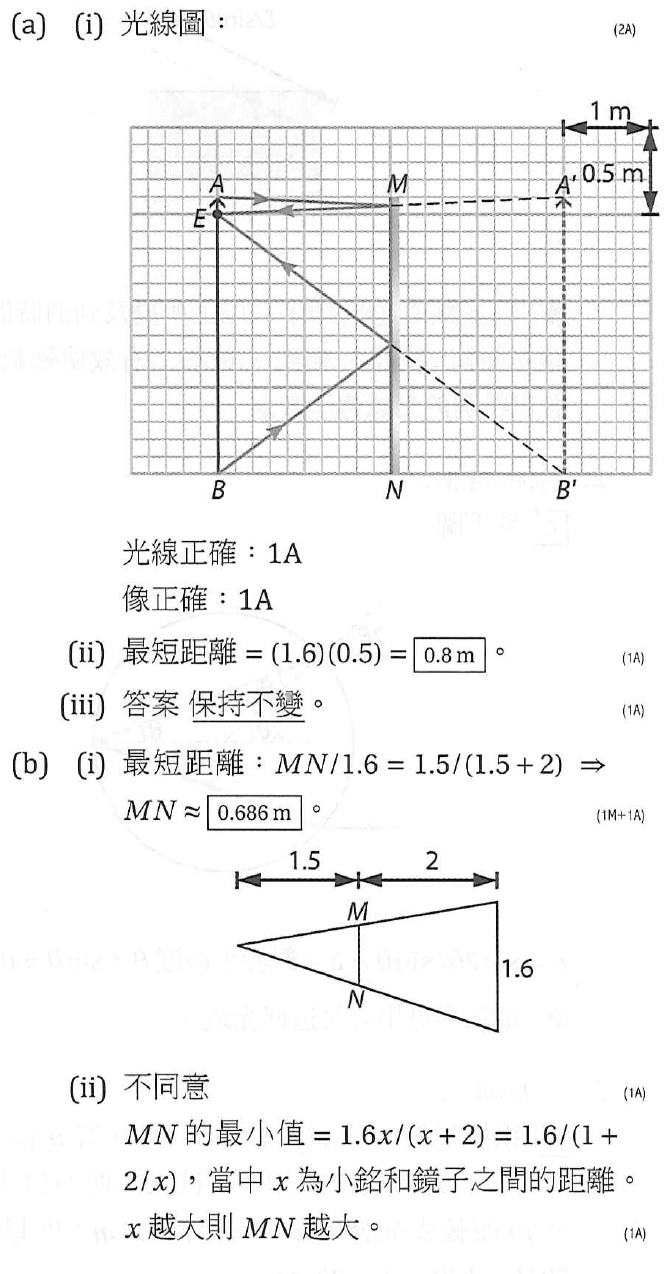
\includegraphics[width=0.75\linewidth]{eo12ieu1n2ge.png}\par}


}
\newprob{lqonec}{
    小新(以箭號AB 表示)站在垂直平面鏡(MN)前 2 m 的位置。已知他高160 cm,眼睛(E) 離地面 150 cm。
    % \\Sam (arrow AB) of height 160 cm is standing 2 m in front of a vertical plane mirror (MN). His eyes (E) are 150 cm above the ground.
    \bigskip
    {\par\centering
        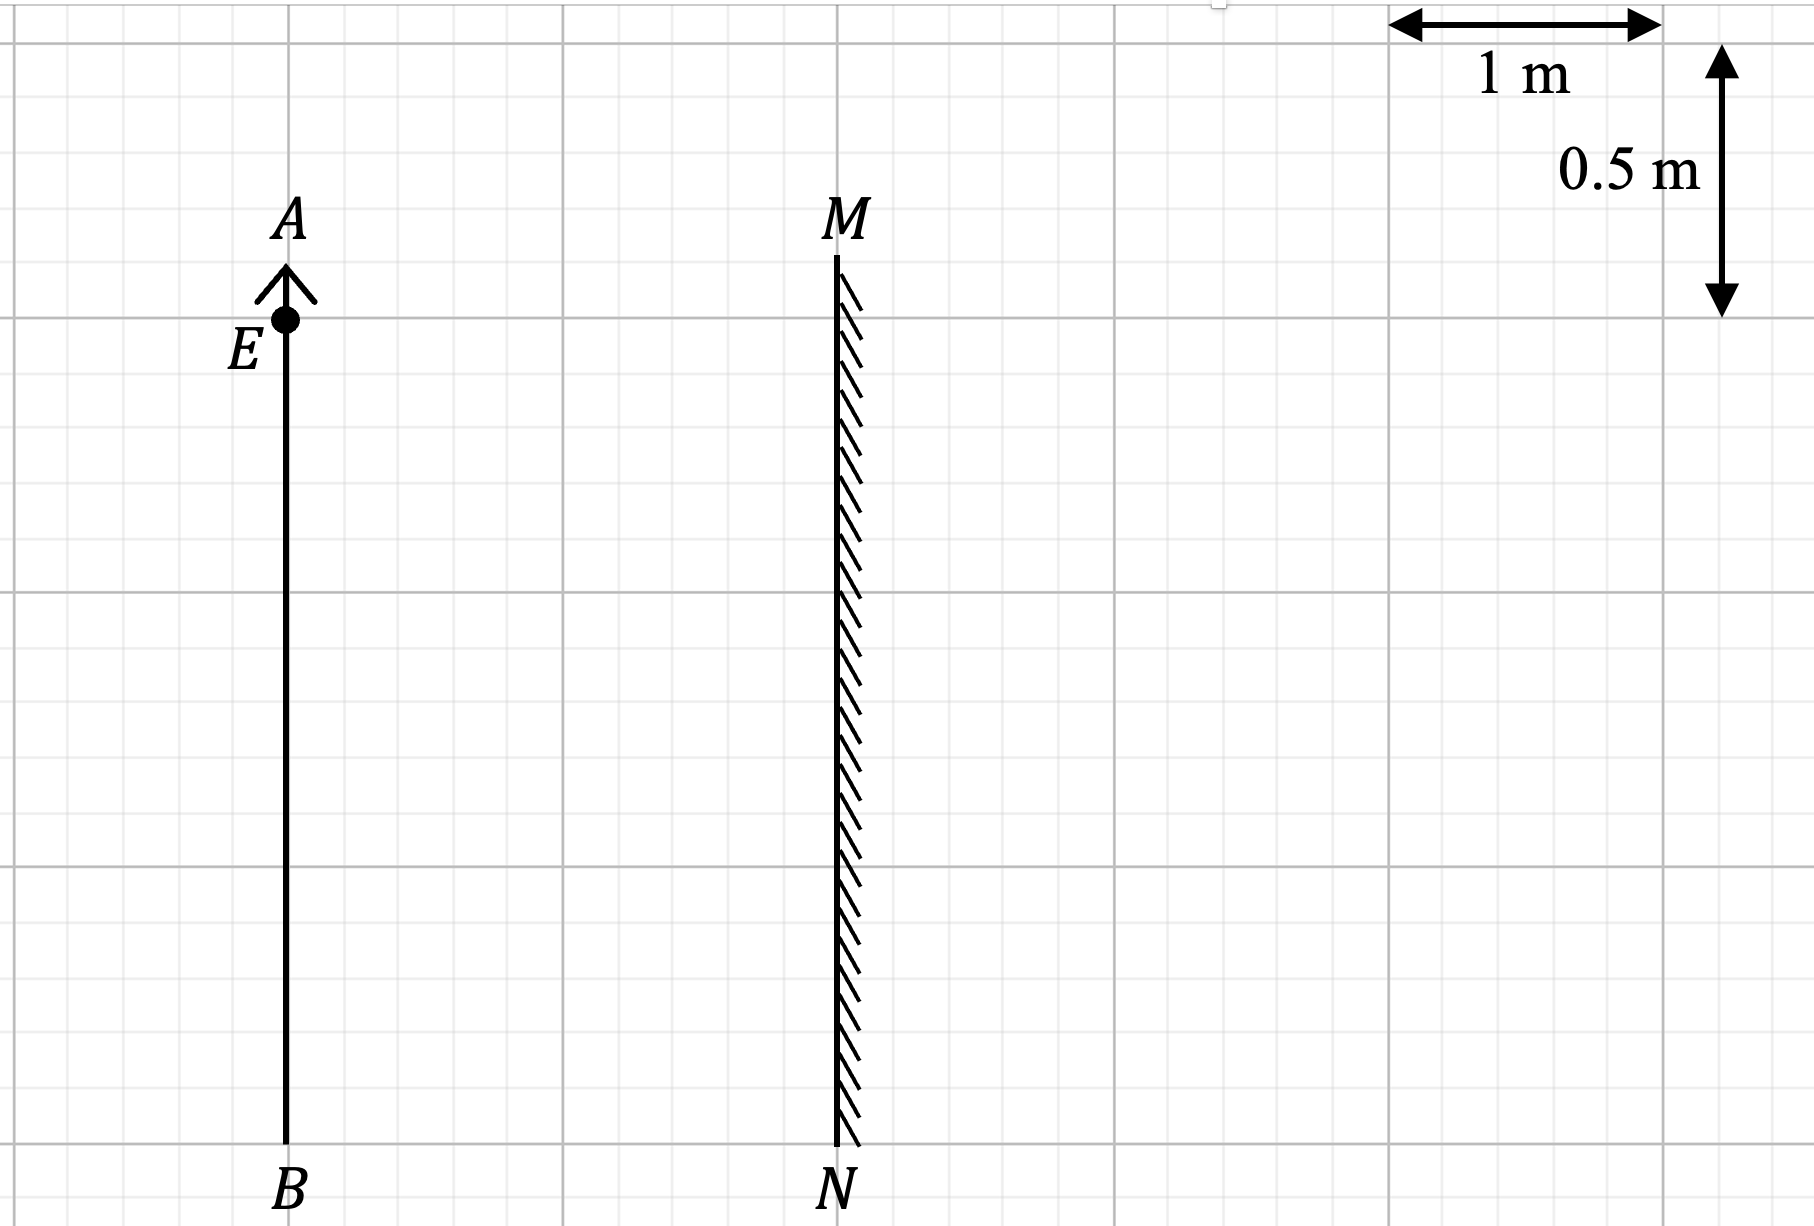
\includegraphics[width=0.75\linewidth]{dq9812us.png}\par}
    \bigskip
    \begin{parts}
        \part \begin{subparts}
            \subpart 試在方格紙上繪畫光線圖,以表示小新 如何在鏡中看見自己的全身像。
            % \\Draw, on the graph paper, a ray diagram to show how Sam sees his whole body in the mirror. 
            \zzh{2}
            \subpart 由此或以其他方法,求鏡子足以讓小新 看見自己的全身像最小長度。
            % \\Hence, or otherwise, find the min. length of the mirror such that Sam can see his whole body. 
            \zzh{1}
            % \dlines{1}
            \subpart 若小新向鏡子走近數步,(ii)的答案會 有何變化?
            % \\How would the answer in (ii) change if Sam moves a few steps towards the mirror? 
            \zzh{1}
            % \dlines{1}
        \end{subparts}

        % \clearpage
        \part 小新的攣生兄弟小銘起初站在小新旁邊。現在小銘向走向小新正前方 0.5 m 處。
        % \\Mike, who is an identical twin of Sam, was standing besides Sam, now is 0.5 m right in front of Sam.
        \begin{subparts}
            \subpart 小銘若要看見小新的全身像,鏡子的最 小長度是多少?
            % \\What is the min. length of the mirror for Mike to see the whole body of Sam?
            \zzh{2}
            % \dlines{1}
            \subpart 小銘認為若他後退數步,(i)的答案會變 小。你同意嗎?試扼要解釋。
            % \\Mike thinks that the answer in (i) would be smaller if he moves a few steps backwards. Do you agree? Explain briefly.
            \zzh{2}
            % \dlines{1}
        \end{subparts}
    \end{parts}

}
{
    {\par\centering
            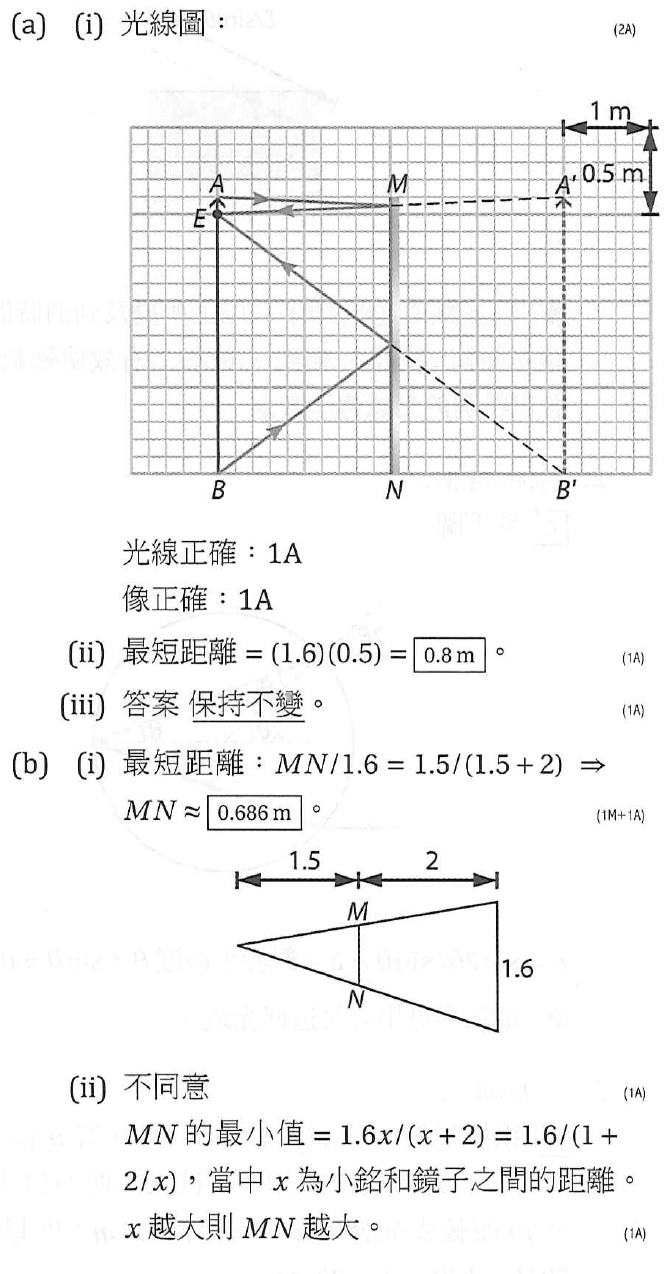
\includegraphics[width=0.75\linewidth]{eo12ieu1n2ge.png}\par}


}

\newprob{mcone}
{
    % aristo p32
    下面的圖示顯示一個男人站在一面平面鏡面前,他可以從頭頂到腳底看到自己的完整影像。\\The diagram below shows a man standing in front of a plane mirror so that he can see his full image from the top of his head to his feet.
        {\par\centering
            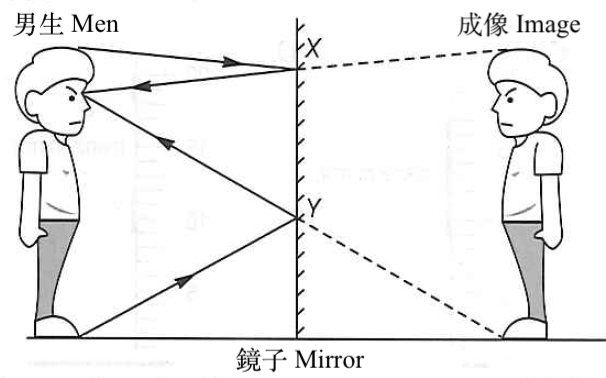
\includegraphics[width=0.35\linewidth]{dewdoiewdjoiwejdiowej.png}\par}
    根據上圖,以下哪些是正確的?\\According to the above diagram, which of the following are correct?
    \begin{statements}
        \task 為了看到他腳的像,這個男人必須低頭望向Y點位置。\\In order to view the image of his feet, the man must look as low as point Y.
        \task 為了看到他頭部的像,這個男人必須抬頭望向X點位置。\\In order to view the image of his head, the man must look as high as point X.
        \task 鏡子在X點和Y點之間的部分以外對於這個男人來說是無用的,因為不會幫助他看到自己完整的像。\\The portions of mirror outside the length between points X and Y are useless for the man to see his full image.
    \end{statements}
    \begin{tasks}
        \task 只有(1)和(2) \tab (1) and (2) only
        \task 只有(1)和(3) \tab (1) and (3) only
        \task 只有(2)和(3) \tab (2) and (3) only
        \task (1), (2) 和 (3)\tab (1), (2) and (3)
    \end{tasks}
}
{\mckey D}
\newprob{mconec}
{
% aristo p32
下面的圖示顯示一個男人站在一面平面鏡面前,他可以從頭頂到腳底看到自己的完整影像。
% \\The diagram below shows a man standing in front of a plane mirror so that he can see his full image from the top of his head to his feet.
{\par\centering
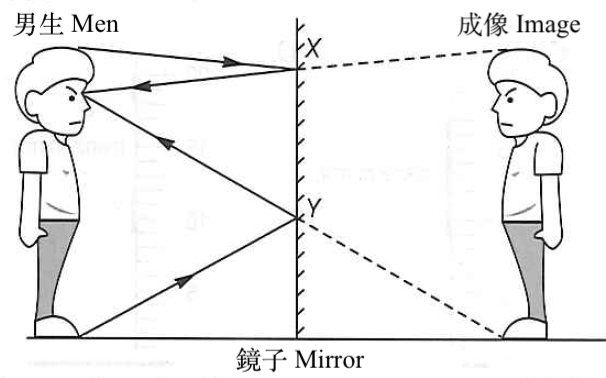
\includegraphics[width=0.35\linewidth]{dewdoiewdjoiwejdiowej.png}\par}
根據上圖,以下哪些是正確的?
% \\According to the above diagram, which of the following are correct?
\begin{statements}
    \task 為了看到他腳的像,這個男人必須低頭望向Y點位置。
    % \\In order to view the image of his feet, the man must look as low as point Y.
    \task 為了看到他頭部的像,這個男人必須抬頭望向X點位置。
    % \\In order to view the image of his head, the man must look as high as point X.
    \task 鏡子在X點和Y點之間的部分以外對於這個男人來說是無用的,因為不會幫助他看到自己完整的像。
    % \\The portions of mirror outside the length between points X and Y are useless for the man to see his full image.
\end{statements}
\begin{tasks}
    \task 只有(1)和(2)
    % \tab (1) and (2) only
    \task 只有(1)和(3)
    % \tab (1) and (3) only
    \task 只有(2)和(3)
    % \tab (2) and (3) only
    \task (1), (2) 和 (3)
    % \tab (1), (2) and (3)
\end{tasks}
}
{\mckey D}

\newprob{mctwozero}{
    \uplevel{\textbf{Question 2 - Question 3}}
    彼得想在牆上安裝一或兩個平面鏡子,好讓他能看到自己的全身,但他希望鏡子的長度盡可能短。他的身高是20單位,眼睛離地面有18單位高。
    \\    Peter would like to fix one or two plane mirrors on the wall so that he can see his whole body in it. But he also wants the mirror(s) to be as short as possible. He is 20 units tall and his eyes are 18 units above the ground.
        {\par\centering
            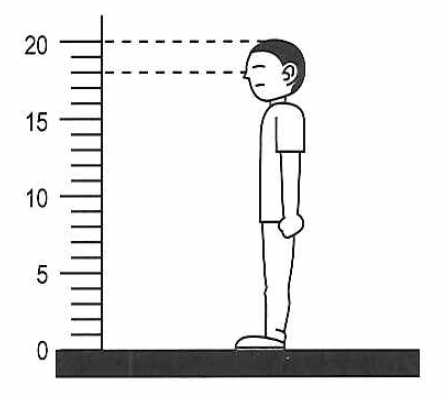
\includegraphics[width=0.25\linewidth]{ddwdkwkdopwekpodew.png}\par}
}{

}
\newprob{mctwozeroc}{
\uplevel{\textbf{Question 2 - Question 3}}
彼得想在牆上安裝一或兩個平面鏡子,好讓他能看到自己的全身,但他希望鏡子的長度盡可能短。他的身高是20單位,眼睛離地面有18單位高。
% \\    Peter would like to fix one or two plane mirrors on the wall so that he can see his whole body in it. But he also wants the mirror(s) to be as short as possible. He is 20 units tall and his eyes are 18 units above the ground.
{\par\centering
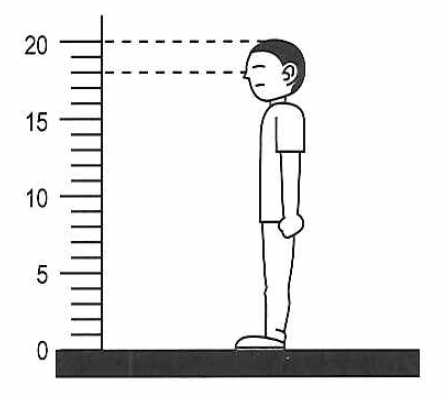
\includegraphics[width=0.25\linewidth]{ddwdkwkdopwekpodew.png}\par}
}{
}

\newprob{mctwoa}{
    % unfinished aristo p32 Q27


    以下哪一種鏡子的佈置最符合彼得的需求?
    \\Which of the following arrangements of the mirror(s) best suits Peter's requirement?
    \begin{tasks}(2)
        \task
        \topalign{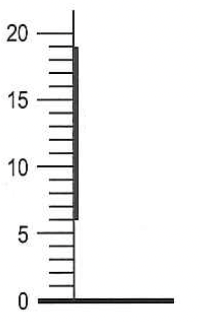
\includegraphics[width=0.3\linewidth]{qdwin89u332u.png}}
        \task
        \topalign{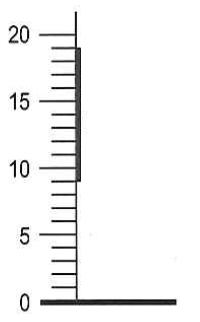
\includegraphics[width=0.3\linewidth]{dowemwejpdoiwejpn23ge.png}}
        \task
        \topalign{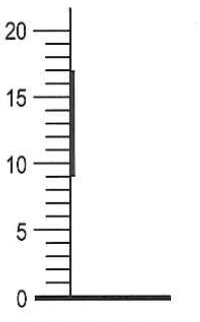
\includegraphics[width=0.3\linewidth]{diwneoipjpu8n3982d.png}}
        \task
        \topalign{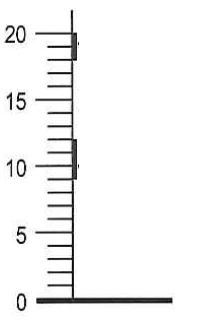
\includegraphics[width=0.3\linewidth]{dweim0939292nd.png}}
    \end{tasks}
}
{\mckey B}
\newprob{mctwoac}{
    % unfinished aristo p32 Q27


    以下哪一種鏡子的佈置最符合彼得的需求?
    % \\Which of the following arrangements of the mirror(s) best suits Peter's requirement?
    \begin{tasks}(2)
        \task
        \topalign{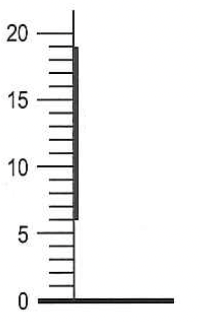
\includegraphics[width=0.3\linewidth]{qdwin89u332u.png}}
        \task
        \topalign{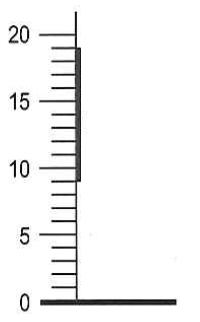
\includegraphics[width=0.3\linewidth]{dowemwejpdoiwejpn23ge.png}}
        \task
        \topalign{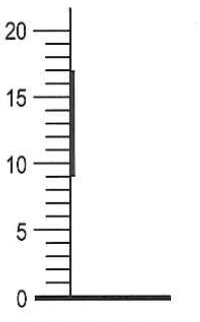
\includegraphics[width=0.3\linewidth]{diwneoipjpu8n3982d.png}}
        \task
        \topalign{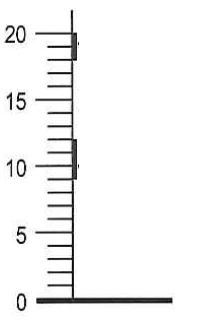
\includegraphics[width=0.3\linewidth]{dweim0939292nd.png}}
    \end{tasks}
}
{\mckey B}

\newprob{mctwob}{
    以下哪一種方式能讓彼得仍然能在鏡子中看到自己的全身影像?
    \\Which of the following would make Peter still can see his whole body image in the mirror?
    \begin{statements}
        \task 他朝鏡子走去。
        \\He walks towards the mirror.
        \task 他從鏡子走開。
        \\He walks away from the mirror.
        \task 他站在鏡子前的椅子上。
        \\He stands on a chair in front of the mirror.
    \end{statements}
    \begin{tasks}
        \task 只有(2) \tab (2) only
        \task 只有(3) \tab (3) only
        \task 只有(1)和(2) \tab (1) and (2) only
        \task 只有(1)和(3) \tab (1) and (3) only
    \end{tasks}
}{\mckey C}
\newprob{mctwobc}{
    以下哪一種方式能讓彼得仍然能在鏡子中看到自己的全身影像?
    % \\Which of the following would make Peter still can see his whole body image in the mirror?
    \begin{statements}
        \task 他朝鏡子走去。
        % \\He walks towards the mirror.
        \task 他從鏡子走開。
        % \\He walks away from the mirror.
        \task 他站在鏡子前的椅子上。
        % \\He stands on a chair in front of the mirror.
    \end{statements}
    \begin{tasks}
        \task 只有(2)
        % \tab (2) only
        \task 只有(3)
        % \tab (3) only
        \task 只有(1)和(2)
        % \tab (1) and (2) only
        \task 只有(1)和(3)
        % \tab (1) and (3) only
    \end{tasks}
}{\mckey C}

\newprob{mcfour}{
    兩面平面鏡 X 和Y 分別水平及垂直放置。兩面鏡從靜止釋放。
    \\Two plane mirrors X and Y are placed horizontally and vertically as shown in the figure. Now both mirrors are released.
        {\par
            \centering
            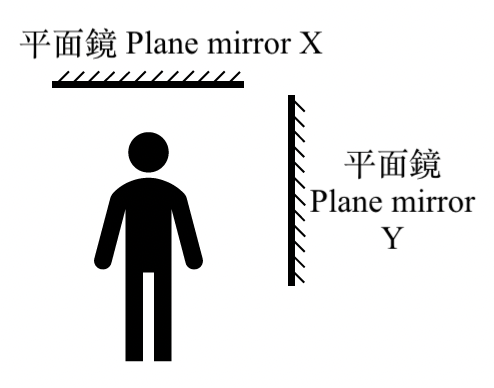
\includegraphics[width=0.25\linewidth]{dq11d23.png}
            \par}
    \par 考慮兩鏡剛釋放一刻,以下哪項是兩鏡中的成像加速度量值?
    \\When both mirrors are released, which of the following is the magnitude of acceleration of images of the mirrors?
    \begin{tasks}
        \task [] \textbf{平面鏡Mirror X}\tab \textbf{平面鏡Mirror Y}
        \task $g$\tab\tab $0$
        \task $g$\tab\tab $g$
        \task $2g$\tab\tab $0$
        \task $2g$\tab\tab $g$
    \end{tasks}
}{C}


\newprob{mcfive}{以下的俯視圖中, ABCD 是一個房間,在牆壁 CD 上掛有一幅掛畫而在牆壁 AB 上有一面垂直的平面鏡(未有在圖中顯示)。
    \\In the top view diagram below, ABCD represents a room. There is a painting hanging on the wall CD, and there is a vertical plane mirror on the wall AB (not shown in the diagram).
        {\par
            \centering
            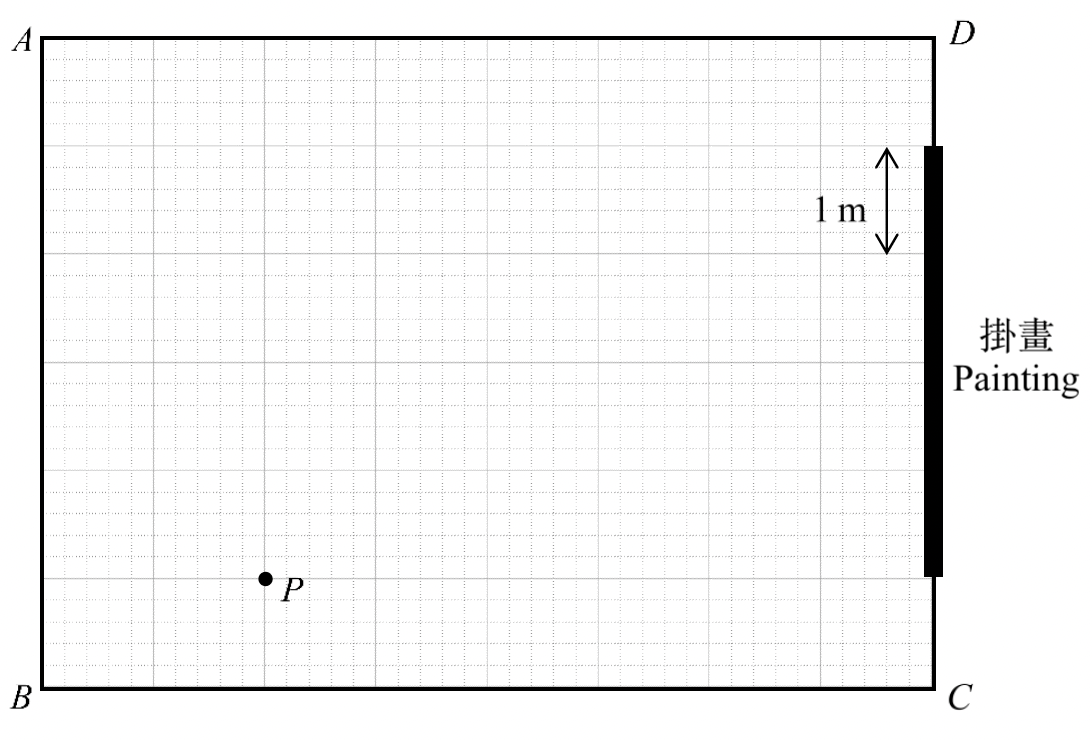
\includegraphics[width=0.45\linewidth]{ddqwdqwd.png}
            \par}
    若一位觀測者在 P 點經前述的平面鏡看到整幅掛畫,求該平面鏡的最小寬度。
    \\If an observer at point P can see the entire painting through the aforementioned plane mirror, find the minimum width of the mirror.
    \begin{tasks}
        \task 2 m
        \task 1 m
        \task 0.8 m
        \task 0.5 m
    \end{tasks}
}{}

\newprob{mcsix}{
    一束光射向一面平面鏡的$O$點,反射後的光線射向屏幕上的$P$點。
    \\A beam of light is projected onto a plane mirror at point O, and the reflected ray is directed towards point P on the screen.
        {\par\centering
            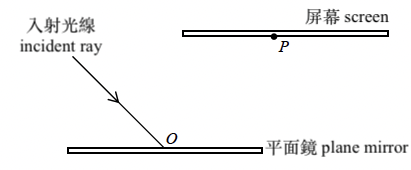
\includegraphics[width=0.5\linewidth]{xnu923.png}\par}
    平面鏡沿$O$點順時針轉動\dg{5},人射光線沿$O$點逆時針轉動了\dg{5}後,光線會射向屏幕上$P$點的左側 還是右側?
    \\After the plane mirror rotates clockwise by \dg{5} around point O, and the person's incident light rotates counterclockwise by \dg{5} around point O, will the light ray be projected to the left or right side of point P on the screen?
    \begin{tasks}
        \task P的左側
        \tab Left side of P
        \task P點
        \tab At P
        \task P的右側
        \tab Right side of P
        \task P的左側還是右側,視乎平面鏡與屏幕的距離。
        \\Depends on the distance between mirror and the screen.
    \end{tasks}
}{C}

% \newprob{mcseven}{
%     在戲劇舞台上,一束光線總是指向天花板上的一個可移動的鏡子,並投射在地板上,如下圖所示。
%     \\On a drama stage, a light beam is always pointed on a movable mirror on the ceiling and projected on the floor as shown.
%         {\par\centering
%             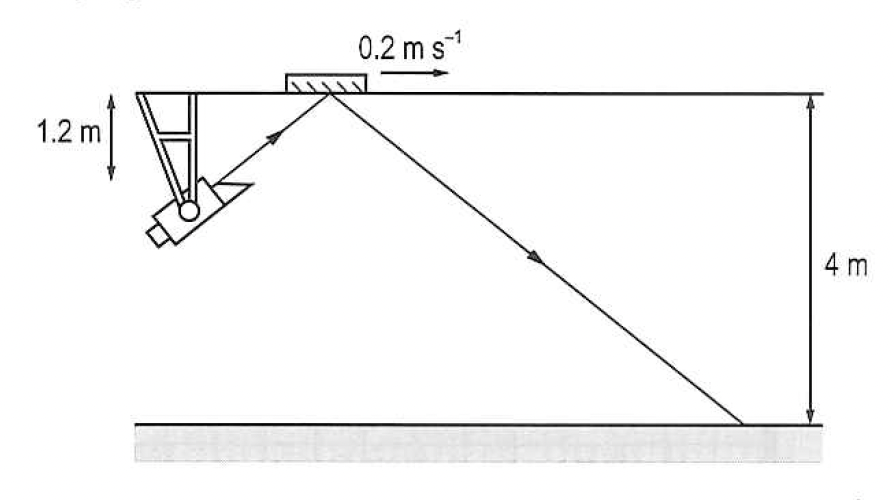
\includegraphics[width=0.5\linewidth]{xn98ef.png}\par}
%     如果可移動鏡子以 \vel{0.2} 的速度遠離光源,請找出地板上的光點的速度。
%     \\If the movable mirror is moving at  \vel{0.2}  away the light source, find the speed of the light spot on the floor.
%     \begin{tasks}
%         \task \vel{0.233}
%         \task \vel{0.489}
%         \task \vel{0.667}
%         \task \vel{0.867}
%     \end{tasks}
% }{}

\newprob{mcseven}{
    在戲劇舞台上,一束光線總是指向天花板上的一個可移動的鏡子,並投射在地板上,如下圖所示。
    \\On a drama stage, a light beam is always pointed on a movable mirror on the ceiling and projected on the floor as shown.
        {\par\centering
            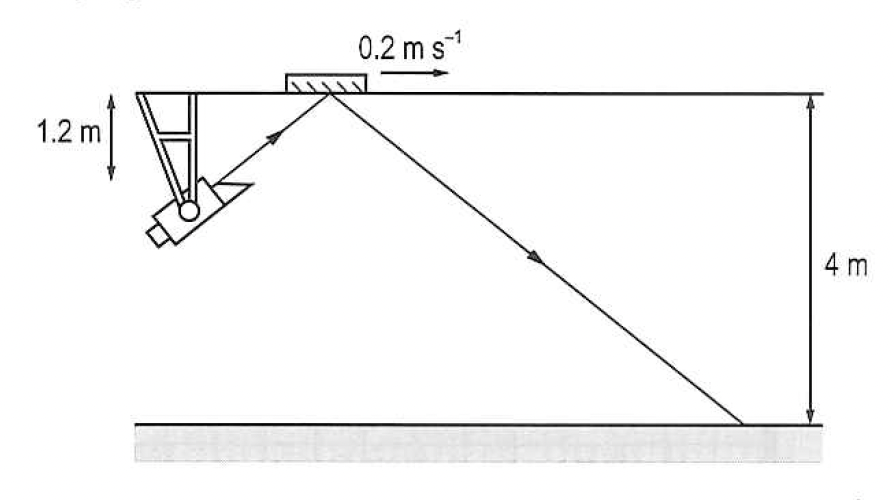
\includegraphics[width=0.5\linewidth]{xn98ef.png}\par}
    如果可移動鏡子以 \vel{0.2} 的速度遠離光源,請找出地板上的光點的速度。
    \\If the movable mirror is moving at  \vel{0.2}  away the light source, find the speed of the light spot on the floor.
    \begin{tasks}
        \task \vel{0.233}
        \task \vel{0.489}
        \task \vel{0.667}
        \task \vel{0.867}
    \end{tasks}
}{\mckey C}
\newprob{mcsevenc}{
在戲劇舞台上,一束光線總是指向天花板上的一個可移動的鏡子,並投射在地板上,如下圖所示。

% \\On a drama stage, a light beam is always pointed on a movable mirror on the ceiling and projected on the floor as shown.
{\par\centering
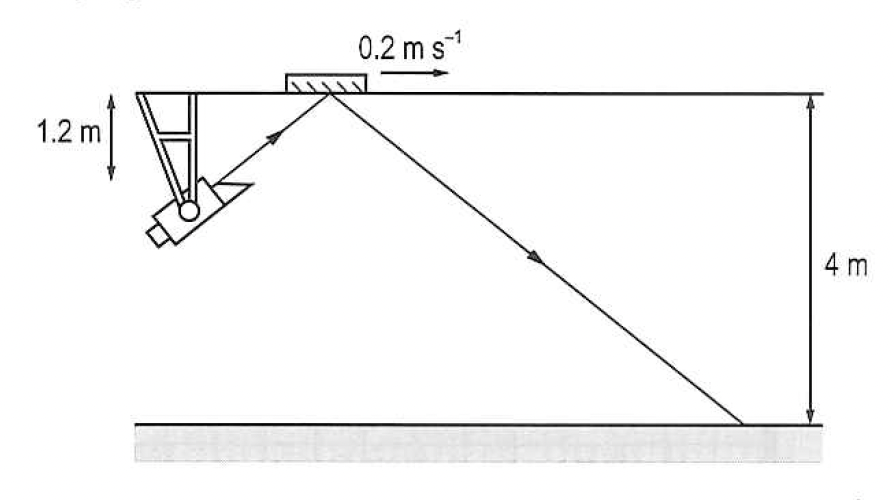
\includegraphics[width=0.5\linewidth]{xn98ef.png}\par}
如果可移動鏡子以 \vel{0.2} 的速度遠離光源,請找出地板上的光點的速度。
% \\If the movable mirror is moving at  \vel{0.2}  away the light source, find the speed of the light spot on the floor.
\begin{tasks}
    \task \vel{0.233}
    \task \vel{0.489}
    \task \vel{0.667}
    \task \vel{0.867}
\end{tasks}
}{\mckey C}


\newprob{1716015735}
{
    % aristo p31 q18
    小明一覺醒來,看著面前的平面鏡中時鐘的影像,誤以為是9:00。下列哪項是可能的實際時間?
    % \\Ming looks at the image of a clock in the plane mirror in front of him and thinks that it is 9 oclock. But it is found to be impossible. What is the correct time?
    \par{\par\centering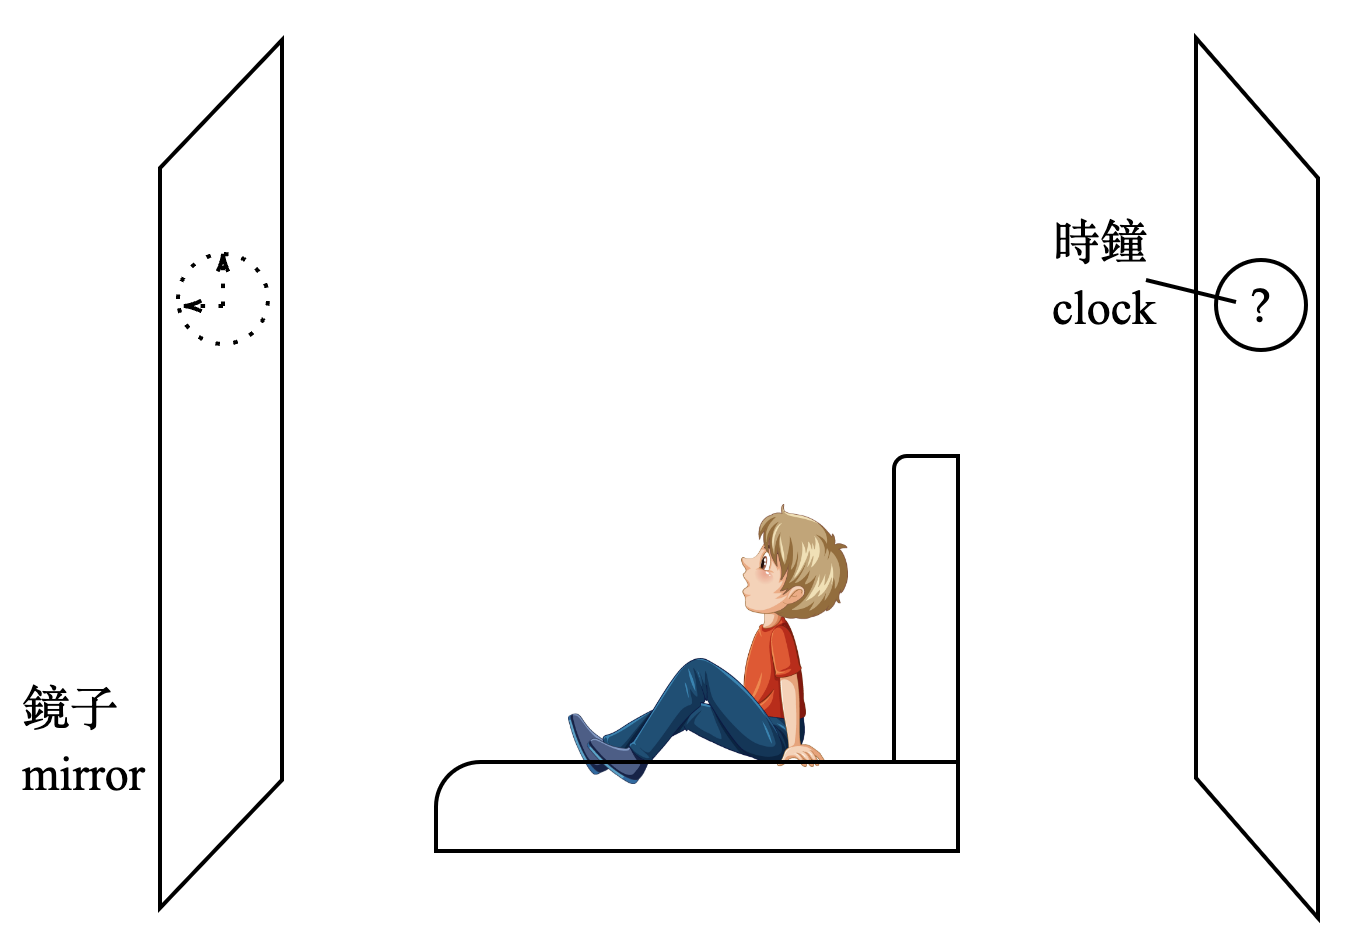
\includegraphics[width=.5\textwidth]{./img/ch1prob_2024-05-18-15-11-35.png}\par}
    \begin{tasks}
        \task 12:15
        \task 12:45
        \task 3:00
        \task 3:45
    \end{tasks}

}{\mckey C}

\newprob{1716016715}
{
    % q21
    平行入射光線如下所示進行漫反射。
    % Parallel incident rays undergo diffuse reflection as shown below.
    \par{\par\centering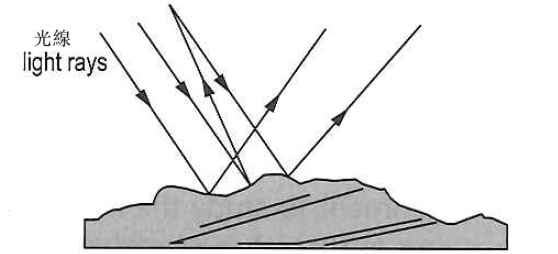
\includegraphics[width=.4\textwidth]{./img/ch1prob_2024-05-18-15-19-42.png}\par}
    % Why do light rays scatter in many different directions from the rough surface? A. Diffuse reflection does not follow the laws of reflection. B. The rough surface can be considered to be made up of a large number of small planar reflecting surfaces positioned at slightly different angles. C. The incident light ray, the normal and the reflected light ray do not fall on the same plane. D. Part of the light hitting on the surface is being absorbed.
    光線為何從粗糙表面上以多種不同方向散射?
    \begin{tasks}
        \task 漫反射不遵循反射定律。
        \task 可以將粗糙表面視為由許多微小的平面反射表面組成,這些表面的角度略有不同。
        \task 入射光線、法線和反射光線不在同一平面上。
        \task 撞擊表面的部分光線被吸收。
    \end{tasks}

}{\mckey B}

\newprob{1716016913}
{
    \topalignc{\par\centering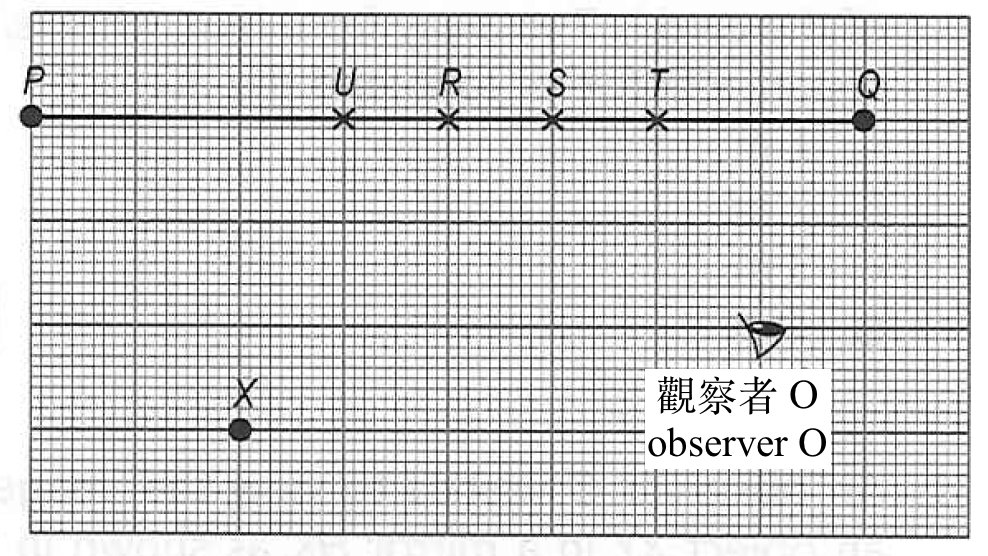
\includegraphics[width=.45\textwidth]{./img/ch1prob_2024-05-18-15-24-27.png}\par}
    面對房間內的牆$PQ$的觀察者$O$希望通過在牆上掛一面小鏡子來看到他後面的物體$X$。他應該把鏡子放在哪裡?
    % An observer O facing the wall PQ inside a room wishes to see object X behind him by hanging a small mirror on the wall. Where should he place the mirror?
    \begin{tasks}
        \task $U$
        \task $R$
        \task $S$
        \task $T$
    \end{tasks}

}{\mckey C}

\newprob{1716017235}
{
    \uplevel{\textbf{Question 7 - Question 8}}
    如下圖所示,有四個乒乓球$P$、$Q$、$R$和$S$放在鏡子前面。
    % Four ping-pong balls, P, Q, R and S are placed in front of a mirror as shown below.
    \par{\par\centering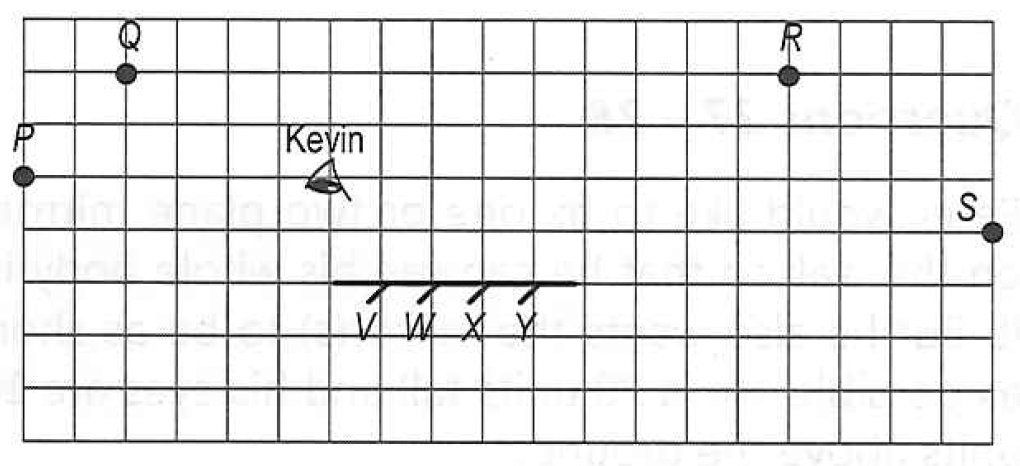
\includegraphics[width=.4\textwidth]{./img/ch1prob_2024-05-18-15-26-34.png}\par}
}{}
\newprob{1716017192}
{
    Kevin可以在鏡子中看到哪個球的影像?
    % Which ball's image can Kevin see in the mirror?
    \begin{tasks}
        \task $P$
        \task $Q$
        \task $R$
        \task $S$
    \end{tasks}

}{\mckey C}

\newprob{1716017372}
{
    第7題中的那個球的光線射向鏡子,然後反射到Kevin的眼睛。光線會在鏡子的哪個位置射向鏡子?
    % The light ray coming from the ball in question 24 hits the mirror and is then reflected to Kevin's eye. At which point would the light ray hit the mirror?
    \begin{tasks}
        \task $V$
        \task $W$
        \task $X$
        \task $Y$
    \end{tasks}

}{\mckey C}

\newprob{1716020039}
{
    % q33
    瑪利站在一組平行平面鏡($M_1$和$M_2$)之間,如下圖所示。她距離$M_1$約 \qty{0.4}{m},距離$M_2$約 \qty{1}{m}。
    % Joyce stands between a set of parallel plane mirrors (Mi and Mz) as shown in the diagram below. She is located at a distance 0.4m from Mi and a distance 1.0 m from M2•
    \par{\par\centering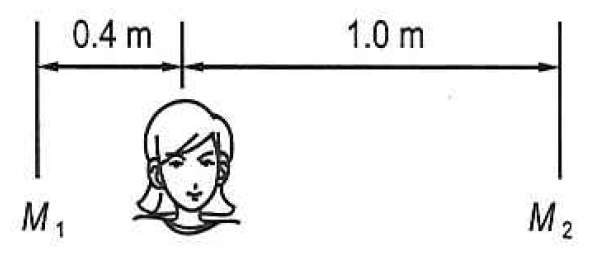
\includegraphics[width=.35\textwidth]{./img/ch1prob_2024-05-18-16-14-20.png}\par}
    鏡子$M_2$後方形成的第二個影像與鏡子$M_2$之間的距離是多少?
    % What is the distance between mirror Mz and the second image formed behind M2?

    \begin{tasks}
        \task \qty{1.0}{m}
        \task \qty{1.4}{m}
        \task \qty{1.8}{m}
        \task \qty{2.8}{m}
    \end{tasks}

}{\mckey C}

\newprob{1716020230}
{
    \uplevel{\textbf{Question 10 - Question 11}}
    一束光線垂直地撞擊在一面平面鏡上。在保持光線盒位置不變的情況下,將鏡子逆時針旋轉 \dg{15} 從$PQ$到$XY$,如下圖所示。
    \bigskip \par{\par\centering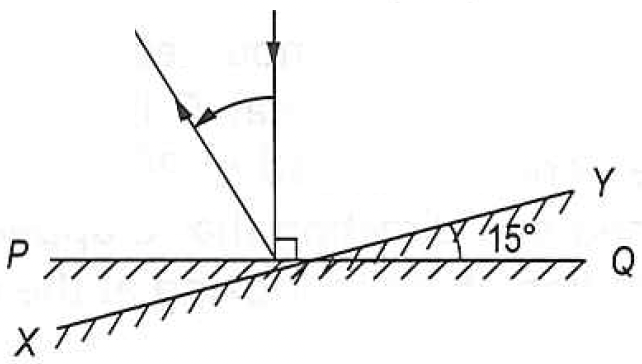
\includegraphics[width=.35\textwidth]{./img/ch1prob_2024-05-18-16-20-23.png}\par} \bigskip
    % A light shield with one slit is placed in front of a ray box. When the ray box is switched on, a ray of light hits on a plane mirror normally. With the ray box kept in the same position, the mirror is rotated anti-clockwise through 15° from PQ to XY as shown below.

}{}

\newprob{1716020465}
{
    以下哪一個(或哪些)也逆時針旋轉了 \dg{15}?
    \begin{statements}
        \task 入射線
        \task 法線
        \task 反射線
    \end{statements}
    \begin{tasks}
        \task 只有(1)
        \task 只有(2)
        \task 只有(1)和(3)
        \task 只有(2)和(3)
    \end{tasks}
}{\mckey B}

\newprob{1716020565}
{
    當鏡子處於$XY$位置時,入射線和反射線之間的角度是多少?
    % When the mirror is at position XY, what is the angle between the incident ray and the reflected ray?
    \begin{tasks}
        \task \dg{7.5}
        \task \dg{15}
        \task \dg{22.5}
        \task \dg{30}
    \end{tasks}


}{\mckey D}